% Copyright © 2018, Loïc Grobol <loic.grobol@gmail.com>
% This document is available under the terms of the Creative Commons Attribution 4.0 International License (CC BY 4.0) (https://creativecommons.org/licenses/by/4.0/)

\RequirePackage{xparse}
\RequirePackage{shellesc}
% Settings
\NewDocumentCommand\myname{}{Loïc Grobol}
\NewDocumentCommand\mylab{}{Lattice, ALMAnaCH}
\NewDocumentCommand\pdftitle{}{Introduction à la fouille de textes}
\NewDocumentCommand\mymail{}{loic.grobol@gmail.com}
\NewDocumentCommand\titlepagetitle{}{\pdftitle}
\NewDocumentCommand\docdate{}{2018}
\NewDocumentCommand\conference{}{M1 Plurital}

\documentclass[hyperref={unicode}, xcolor={svgnames}]{beamer}
\usetheme[sectionpage=progressbar,
          subsectionpage=progressbar,
          progressbar=frametitle]{metropolis}
    \definecolor{accent}{RGB}{51, 34, 136}
    \setbeamercolor{alerted text}{fg=accent}
    \makeatletter
        \setlength{\metropolis@progressinheadfoot@linewidth}{1pt}
    \makeatother
\usepackage{appendixnumberbeamer}

% Highlight colour palette
\definecolor{highlight0}{RGB}{51, 34, 136}
\definecolor{highlight1}{RGB}{136, 204, 238}
\definecolor{highlight2}{RGB}{68, 170, 153}
\definecolor{highlight3}{RGB}{17, 119, 51}
\definecolor{highlight4}{RGB}{153, 153, 51}
\definecolor{highlight5}{RGB}{221, 204, 119}
\definecolor{highlight6}{RGB}{204, 102, 119}
\definecolor{highlight7}{RGB}{136, 34, 85}
\definecolor{highlight8}{RGB}{170, 68, 153}

% Use non-standard fonts
\usefonttheme{professionalfonts}
\setsansfont[BoldFont={Fira Sans SemiBold}, ItalicFont={Fira Sans Book Italic}]{Fira Sans Book}
\setmonofont[Scale=0.9]{Fira Mono}

% Notes on left screen
% \usepackage{pgfpages}
% \setbeameroption{show notes on second screen=left}


\usepackage{polyglossia}
	\setmainlanguage{french}
    \setotherlanguage{english}

    % PATCH: fix spacing in monospaced text
    \usepackage{xpatch}
    \makeatletter
        \xapptocmd\ttfamily{\nofrench@punctuation}{}{}
    \makeatother

\usepackage[math-style=french]{unicode-math}
	\setmathfont{XITS Math}
\usepackage{newunicodechar}
	\newunicodechar{√}{\sqrt}

\usepackage{tabu}
\usepackage{booktabs}
\usepackage{siunitx}
\usepackage{multicol}
\usepackage{ccicons}
\usepackage{bookmark}
\usepackage{caption}
    \captionsetup{skip=1ex}

\usepackage{csquotes}
\usepackage{tikz}
	\NewDocumentCommand{\textnode}{O{}mm}{\tikz[remember picture, baseline=(#2.base), inner sep=0pt]{\node[#1] (#2) {#3};}}
	\tikzset{
		invisible/.style={opacity=0},
		visible on/.style=,
		alt/.code args={<#1>#2#3}{%
		\alt<#1>{\pgfkeysalso{#2}}{\pgfkeysalso{#3}} % \pgfkeysalso doesn't change the path
		},
	}
	\usepackage{tikz-qtree}
    \usepackage{tkz-graph}
    \usepackage{pgfplots}
        \pgfplotsset{compat=1.15}
        \pgfplotsset{colormap={SRON}{rgb255=(61,82,161) rgb255=(255,250,210) rgb255=(174,28,62)}}


	\usetikzlibrary{positioning, calc, shapes, shapes.geometric, intersections}

    % Do evil things with soft path
    % From <https://tex.stackexchange.com/a/301364/8547>
    \makeatletter
        \def\@appendnamedsoftpath#1{%
            \pgfsyssoftpath@getcurrentpath\@temppatha
            \expandafter\let\expandafter\@temppathb\csname tikz@intersect@path@name@#1\endcsname
            \expandafter\expandafter\expandafter\def\expandafter\expandafter\expandafter\@temppatha\expandafter\expandafter\expandafter{\expandafter\@temppatha\@temppathb}%
            \pgfsyssoftpath@setcurrentpath\@temppatha
        }
        \def\@appendnamedpathforactions#1{%
            \pgfsyssoftpath@getcurrentpath\@temppatha
            \expandafter\let\expandafter\@temppathb\csname tikz@intersect@path@name@#1\endcsname
            \expandafter\def\expandafter\@temppatha\expandafter{\csname @temppatha\expandafter\endcsname\@temppathb}%
            \let\tikz@actions@path\@temppatha
        }

        \tikzset{
            use path for main/.code={%
                \tikz@addmode{%
                    \expandafter\pgfsyssoftpath@setcurrentpath\csname tikz@intersect@path@name@#1\endcsname
                }%
            },
            append path for main/.code={%
                \tikz@addmode{%
                    \@appendnamedsoftpath{#1}%
                }%
            },
            use path for actions/.code={%
                \expandafter\def\expandafter\tikz@preactions\expandafter{\tikz@preactions\expandafter\let\expandafter\tikz@actions@path\csname tikz@intersect@path@name@#1\endcsname}%
            },
            append path for actions/.code={%
                \expandafter\def\expandafter\tikz@preactions\expandafter{\tikz@preactions
                \@appendnamedpathforactions{#1}}%
            },
            use path/.style={%
                use path for main=#1,
                use path for actions=#1,
            },
            append path/.style={%
                append path for main=#1,
                append path for actions=#1
            }
        }
    \makeatother

    % TikZ externalisation
    \usetikzlibrary{external}
    % Make externalization work with overlays, stolen from <https://tex.stackexchange.com/a/119440/8547>
    \makeatletter
        \newcommand*{\overlaynumber}{\number\beamer@slideinframe}
        \tikzset{
            beamer externalizing/.style={
                execute at end picture={%
                    \tikzifexternalizing{%
                        \ifbeamer@anotherslide
                            \pgfexternalstorecommand{\string\global\string\beamer@anotherslidetrue}
                        \fi
                    }{}
                }
            },
            every picture/.style={beamer externalizing}
        }
        \let\orig@tikzsetnextfilename=\tikzsetnextfilename
        \renewcommand\tikzsetnextfilename[1]{\orig@tikzsetnextfilename{#1-\overlaynumber}}
    \makeatother
    % Create the `tikzpics/` folder if it does not exist
    \ShellEscape{mkdir tikzpics}
    % Only externalise pictures on demand (to avoid messing up with metropolis theme)
    \tikzset{
        external/export=false,
        external/prefix=tikzpics/
    }
    \tikzexternalize

\usepackage{listings}
\renewcommand{\lstlistingname}{Example}

    \makeatletter
    	\lstset{
    		basicstyle=\ttfamily\lst@ifdisplaystyle\footnotesize\fi,
    		columns=fullflexible,
    		showstringspaces=false,
    		commentstyle=\color{gray}\upshape
    	}
    \makeatother

	\lstdefinelanguage{XML}{
	    morestring=[s]{"}{"},
	    morecomment=[s]{?}{?},
	    morecomment=[s]{!--}{--},
	    moredelim=[s][\color{black}]{>}{<},
	    moredelim=[s][\color{highlight0}]{\ }{=},
	    stringstyle=\color{highlight3},
	    identifierstyle=\color{highlight7}
	}

\usepackage[style=authoryear, block=ragged, doi=false, isbn=false]{biblatex}
    \AtEveryBibitem{
        \ifentrytype{online}
        {} {
            \iffieldequalstr{howpublished}{online}
            {
                \clearfield{howpublished}
            } {
                \clearfield{urlyear}\clearfield{urlmonth}\clearfield{urlday}
            }
        }
    }

	\addbibresource{biblio.bib}

% Compact bibliography style
\setbeamertemplate{bibliography item}[text]

\AtEveryBibitem{
    \clearfield{series}
    \clearfield{pages}
    \clearlist{publisher}
    \clearname{editor}
    \clearlist{location}
}
\renewcommand*{\bibfont}{\tiny}

\usepackage{hyperxmp}	% XMP metadata

\usepackage[type={CC},modifier={by},version={4.0}]{doclicense}

\usepackage{todonotes}
\let\todox\todo
\renewcommand\todo[1]{\todox[inline]{#1}}

\title{\titlepagetitle}
\author{\textbf{\myname}}
\institute{}
\date{\conference\\\docdate}

\titlegraphic{\ccby}

% Tikz styles

% Schémas de tâches
\tikzset{
    >=stealth,
    data/.style={draw, ellipse},
    program/.style={draw, rectangle},
    true scale/.style={scale=#1, every node/.style={transform shape}}
}

% Styles des heatmap pour les moyennes
\pgfplotsset{
    meanheatmap/.style={
        colorbar, colormap name=SRON,
        view={0}{90},
        samples=100,
        domain=0:1,
        min=0, max=1
    }
}


% Commands spécifiques
\NewDocumentCommand\shorturl{ O{https} O{://} m }{%
    \href{#1#2#3}{\nolinkurl{#3}}%
}


% ██████   ██████   ██████ ██    ██ ███    ███ ███████ ███    ██ ████████
% ██   ██ ██    ██ ██      ██    ██ ████  ████ ██      ████   ██    ██
% ██   ██ ██    ██ ██      ██    ██ ██ ████ ██ █████   ██ ██  ██    ██
% ██   ██ ██    ██ ██      ██    ██ ██  ██  ██ ██      ██  ██ ██    ██
% ██████   ██████   ██████  ██████  ██      ██ ███████ ██   ████    ██


\begin{document}
\pdfbookmark[2]{Title}{title}

\begin{frame}[plain]
	\titlepage
\end{frame}

\lecture{Introduction à la fouille de textes}{2018-01-15}
\begin{frame}{Informations pratiques}
    \begin{description}[Contact]
        \item[Où] Salle Benveniste, ILPGA, 9 Rue des Bernardins, 75005 Paris
        \item[Quand] Le lundi de 14h à 16h (voir le calendrier de Paris 3 pour les dates)
        \item[Contact] \shorturl[mailto][:]{loic.grobol@gmail.com}{loic.grobol@gmail.com}
        \item[Web] {\small\shorturl{loicgrobol.github.io/intro-fouille-textes}}
    \end{description}
\end{frame}

\begin{frame}{Organisation}
    \begin{description}[Évaluation]
        \item[Poly] À lire d'une fois sur l'autre :
                    {\footnotesize\shorturl[https]{loicgrobol.github.io/intro-fouille-textes/poly/poly.pdf}}
        \item[Cours] Exemples, exercices, expérimentations, explications
        \item[Évaluation] en contrôle continu
            \begin{description}
                \item[Partiel] en semaine 13 (2018-04-23) → \SI{50}{\percent}
                \item[Projet] → \SI{50}{\percent}
            \end{description}
    \end{description}
\end{frame}

\begin{frame}{Projet final}
    « Utiliser des programmes d'apprentissage automatique pour un tâche de classification de textes »
    \begin{itemize}
        \item Définir le sujet
        \item Constituer le corpus de travail
        \item Transformation du texte en données utilisables par Weka
        \item Expérimentations
        \item Compte-rendu
    \end{itemize}
\end{frame}

\begin{frame}{Weka ?}
    Une suite de logiciels pour l'apprentissage automatique avec une interface graphique
    \begin{itemize}
        \item \shorturl{www.cs.waikato.ac.nz/ml/weka}
        \item À installer dès que possible sur votre machine
        \item Si possible, venir avec votre PC portable pour pouvoir suivre les expérimentations en cours
    \end{itemize}
\end{frame}

% ██ ███    ██ ████████ ██████   ██████  ██████  ██    ██  ██████ ████████ ██  ██████  ███    ██
% ██ ████   ██    ██    ██   ██ ██    ██ ██   ██ ██    ██ ██         ██    ██ ██    ██ ████   ██
% ██ ██ ██  ██    ██    ██████  ██    ██ ██   ██ ██    ██ ██         ██    ██ ██    ██ ██ ██  ██
% ██ ██  ██ ██    ██    ██   ██ ██    ██ ██   ██ ██    ██ ██         ██    ██ ██    ██ ██  ██ ██
% ██ ██   ████    ██    ██   ██  ██████  ██████   ██████   ██████    ██    ██  ██████  ██   ████


\section*{Introduction}

\begin{frame}{La fouille de données}
    Tout commença dans les années 90…
    \begin{itemize}
        \item Généralisation des ordinateurs personnels
        \item Augmentation de leurs capacités de mémorisation et de traitement
        \item[→] Il devient possible de traiter rapidement de grandes quantités d'informations
    \end{itemize}
    Le terme \alert{fouille de données} désigne l'ensemble des techniques permettant de prendre des décisions pertinentes à partir de l'analyse de données massives.
\end{frame}

\begin{frame}{La fouille de données}
    Intéressant et rentable
    \begin{itemize}
        \item Pour les banques et les assurances
            \begin{itemize}
                \item[→] Fiabilité d'un crédit, d'une garantie…
            \end{itemize}
        \item Pour la médecine
            \begin{itemize}
                \item[→] Efficacité d'un traitement, propagation d'une épidémie…
            \end{itemize}
        \item Pour la vente et le marketing
            \begin{itemize}
                \item[→] Cibler des publicités, étudier un marché…
            \end{itemize}
        \item …
    \end{itemize}
\end{frame}

\begin{frame}{Particularités innovantes}
    Par rapport à l'IA traditionnelle, on privilégie
    \begin{itemize}
        \item \alert{La masse de données} plutôt que les compétences expertes
        \item \alert{Les méthodes numériques} plutôt que symboliques
        \item Une démarche \alert{inductive} plutôt que déductive
    \end{itemize}
    Et cette tendance se généralise depuis à l'ensemble des domaines de l'informatique.

    À lire : \citetitle{church2011pendulum} \parencite{church2011pendulum}
\end{frame}

\begin{frame}{La fouille de textes}
    Applications de la fouille de données au TAL et vice-versa pour le traitement des données linguistiques massives.

    \begin{itemize}
        \item Le web 2.0 se démocratise au même moment
        \item C'est une formidable source de données linguistiques
        \item Mais elles sont en général spontanées et potentiellement mal formées
    \end{itemize}

    Et le TAL traditionnel, et en particulier
    \begin{itemize}
        \item Automates
        \item Grammaires formelles
        \item Représentations logiques
    \end{itemize}
    ne sont pas adaptées.
\end{frame}

\begin{frame}{Un changement de paradigme}
    En fouille de textes, par rapport au TAL traditionnel
    \begin{itemize}
        \item On privilégie les analyses de surface
        \item On s'appuie sur la quantité des données pour compenser leur hétérogénéité
        \item On réduit les ambitions : pas question d'accéder au sens profond des textes
    \end{itemize}

    L'objectif est de traiter efficacement quelques \alert{tâches} précises et limitées.
\end{frame}

\begin{frame}{Sommaire}
    La suite de ce cours est articulée en deux parties
    \begin{itemize}
        \item Les tâches élémentaires de la fouille de textes
         \begin{itemize}
             \item Qu'est-ce qu'une tâche ?
             \item Quelles sont les tâches élémentaires ?
             \item Combiner des tâches élémentaires
         \end{itemize}
        \item Une tâche particulière : la classification de textes
    \end{itemize}
\end{frame}

% ████████  █████   ██████ ██   ██ ███████ ███████
%    ██    ██   ██ ██      ██   ██ ██      ██
%    ██    ███████ ██      ███████ █████   ███████
%    ██    ██   ██ ██      ██   ██ ██           ██
%    ██    ██   ██  ██████ ██   ██ ███████ ███████

\section{Les tâches élémentaires de la fouille de textes}

\subsection{Notion de tâche}

\begin{frame}{Introduction}
    On traite du concept de \textit{tâche} au sens de l'informatique : spécification d'un programme qui mime une compétence humaine précise.

    \begin{itemize}
        \item Définition très large
            \begin{itemize}
                \item[→] « Tenir une conversation par écrit en se faisant passer pour un être humain » convient
            \end{itemize}
        \item En pratique on a des ambitions plus modestes
        \item Mais on est encore loin de les satisfaire !
         \begin{itemize}
             \item Notre mesure du succès est « s'approcher le plus possible d'une solution de référence validée par un humain »
         \end{itemize}
    \end{itemize}
 \end{frame}

\begin{frame}{Caractérisation}
    \begin{itemize}
        \item Chaque tâche a une visée applicative précise et autonome
        \item Elle est caractérisée par ses entrées, ses sorties et les ressources auxquelles elle fait appel
    \end{itemize}

    \begin{figure}
        \tikzset{external/export=true}
        \begin{tikzpicture}[>=stealth]
            \node[data] (in) {Entrée};
            \node[program, right=1cm of in, text width=10ex] (prog) {Programme réalisant la tâche};
            \node[data, right=1.5cm of prog] (out) {Résultat};
            \node[data, below=1cm of prog] (res) {Ressources};
            \draw[->] (in) -- (prog);
            \draw[->] (prog) -- (out);
            \draw[->] (res) -- (prog);
        \end{tikzpicture}
    \end{figure}

    On peut considérer chaque tâche comme une boîte noire : la façon dont le programme fonctionne ne nous intéresse pas ici.
\end{frame}

\begin{frame}{Quelques exemples de tâches}
    \begin{enumerate}
        \item Détecter les spams dans un ensemble d'emails
        \item Trouver dans le catalogue d'une bibliothèque de ouvrages qui traitent de l'art macabre au XVème siècle
        \item Trouver un site internet qui vend des ordinateurs portable sans système d'exploitation
        \item Déterminer le nom du héros et des principaux protagonistes d'un texte narratif
        \item Découper la transcription d'un discours en parties thématiques
        \item Déterminer les symptômes présentés par un patient à partir d'un rapport clinique
        \item Repérer dans un ensemble de tweets ceux qui sont sarcastiques ou ironiques
    \end{enumerate}
\end{frame}

\begin{frame}[fragile]{Schéma général d'une tâche}
    \begin{figure}
        \tikzset{external/export=true}
        \begin{tikzpicture}[>=stealth]
            \tikzset{accent on/.style={alt={#1{draw=accent, text=accent, thick}{draw}}}}
            \node[ellipse, accent on=<2>] (in) {Entrée};
            \node[right=1cm of in, text width=10ex, accent on=<3>] (prog) {Programme réalisant la tâche};
            \node[ellipse, accent on=<2>, right=1.5cm of prog] (out) {Résultat};
            \node[ellipse, accent on=<2>, below=1cm of prog] (res) {Ressources};
            \draw[->] (in) -- (prog);
            \draw[->] (prog) -- (out);
            \draw[->] (res) -- (prog);
        \end{tikzpicture}
        \caption{Schéma général d'une tâche}
    \end{figure}
    \only<2->{
    Dans ce schéma
        \begin{itemize}
            \item<2-> Les \alert<2>{données} sont figurées par des ellipses.
            \item<3-> Le \alert<3>{programme} réalisant la tâche est figuré par un rectangle.
        \end{itemize}
    }
\end{frame}

\begin{frame}{Entrées ou ressources ?}
    Le critère qu'on retiendra en pratique est la mutabilité
    \begin{itemize}
        \item Une ressource est une donnée stable qui n'est pas modifiée entre deux exécutions du programme
        \item Une donnée d'entrée change à chaque exécution du programme
    \end{itemize}
\end{frame}

\begin{frame}{Exemples}
    Pour les tâches suivantes, identifier entrées et sorties et proposer des ressources
    \begin{enumerate}
        \item Détecter les spams dans un ensemble d'emails
        \item Déterminer le nom du héros et des principaux protagonistes d'un texte narratif
        \item Découper la transcription d'un discours en parties thématiques
        \item Repérer dans un ensemble de tweets ceux qui sont sarcastiques ou ironiques
    \end{enumerate}
\end{frame}

\begin{frame}{Données}
    On peut regrouper grossièrement les données utilisées en fouille de texte dans trois catégories
    \begin{itemize}
        \item Les données tabulaires
        \item Les textes bruts
        \item Les documents semi-structurés
    \end{itemize}
\end{frame}

\begin{frame}{Données tabulaires}
    \begin{figure}
        \includegraphics<1>[width=\textwidth, height=0.75\textheight, keepaspectratio]{pics/tab_weka.png}
        \includegraphics<2>[width=\textwidth, height=0.4\textheight, keepaspectratio]{pics/tab_weka.png}
        \caption{Données tabulaires dans Weka}
    \end{figure}
    \alt<1>{
        \vspace{-1\baselineskip}
        {\tiny Exemple Weka \texttt{weater.numeric} : peut-on jouer au tennis aujourd'hui ?}
    }{
        C'est le type de données traditionnellement utilisé en fouille de données
        \begin{itemize}
            \item L'ordre des lignes est arbitraire
            \item L'ordre des colonnes est arbitraire, sauf éventuellement pour la dernière
        \end{itemize}
    }
\end{frame}

\begin{frame}[fragile=singleslide]{Textes bruts}
    \begin{figure}
        \begin{lstlisting}[gobble=12, basicstyle=\ttfamily\small]
            et comment est-ce qu'on fait une omelette est-ce que vous
            pourriez m'expliquer
            comment on fait une omelette ?
            ah une omelette oui bien sûr
            je casse des oeufs
            oui oui
            je les mets dans un récipient
            je mets du sel et du poivre directement
            je bats bon je prépare ma poêle je mets du beurre hein ?
        \end{lstlisting}
        \caption{Exemple de texte brut}
    \end{figure}
    \vskip0pt plus 1fill
    {\tiny Extrait du corpus ANCOR \parencite{muzerelle2013ANCOR}}
\end{frame}

\begin{frame}{Textes bruts}
    \alert{Tous} les caractères représentables sont susceptibles d'en faire partie
    \begin{figure}
        
\includegraphics[width=\textwidth, height=0.8\textheight, keepaspectratio]{pics/raw_emoji.png}
        \caption{Texte brut avec caractères spéciaux}
    \end{figure}
    \vskip0pt plus 1fill
    {\tiny @Biolojical@twitter : \shorturl{twitter.com/biolojical/status/949344635310059520}}
\end{frame}

\begin{frame}[fragile=singleslide]{Documents semi-structuré}
    Cas typique : XML et HTML
    \begin{figure}
        \begin{lstlisting}[gobble=12, language=XML]
            <table>
                <tr><th>produit</th><th>marque</th><th>prix en euros</th></tr>
                <tr><td>ordinateur portable</td><td>truc</td><td>800</td></tr>
                <tr><td>tablette</td><td>machin</td><td>200</td></tr>
            </table>
        \end{lstlisting}
        \caption{HTML vu comme texte brut}
    \end{figure}
    On peut le considérer comme du texte brut où chaque balise (\lstinline[language=XML]{<td>}, \lstinline[language=XML]{</tr>}…) compte comme un seul caractère.
\end{frame}

\begin{frame}[fragile=singleslide]{Documents semi-structuré}
    On peut aussi le considérer comme un arbre
    \begin{figure}
        \tikzset{external/export=true}
        \begin{tikzpicture}[font=\tiny]
            \tikzset{level distance=2em, sibling distance=1ex}

            \Tree[.{\lstinline[language=XML]{<table>}}
                [.{\lstinline[language=XML]{<tr>}}
                    [.{\lstinline[language=XML]{<th>}} produit ]
                    [.{\lstinline[language=XML]{<th>}} marque ]
                    [.{\lstinline[language=XML]{<th>}} {prix en euros} ]
                ]
                [.{\lstinline[language=XML]{<tr>}}
                    [.{\lstinline[language=XML]{<td>}} {ordinateur portable} ]
                    [.{\lstinline[language=XML]{<td>}} truc ]
                    [.{\lstinline[language=XML]{<td>}} 800 ]
                ]
                [.{\lstinline[language=XML]{<tr>}}
                    [.{\lstinline[language=XML]{<td>}} tablette ]
                    [.{\lstinline[language=XML]{<td>}} machin ]
                    [.{\lstinline[language=XML]{<td>}} 200 ]
                ]
            ]
        \end{tikzpicture}
        \caption{HTML vu comme un arbre}
    \end{figure}
\end{frame}

\begin{frame}{Documents semi-structurés}
    Et ils admettent dans certains cas des représentations supplémentaires
    \begin{figure}
        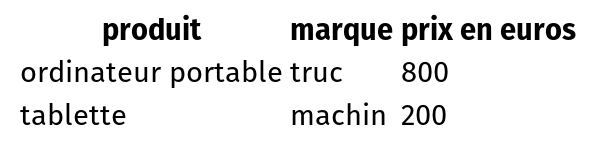
\includegraphics[width=\textwidth, height=0.8\textheight, keepaspectratio]{pics/html_firefox.png}
        \caption{Représentation du code précédent dans un navigateur}
    \end{figure}
    \vskip0pt plus 1fill
    {\tiny Représentation standard dans Mozilla Firefox \shorturl{www.mozilla.org/firefox/}}
\end{frame}

\begin{frame}{Les ressources}
    \begin{quote}
        {\only<2>{\small}Toute donnée ou programme disponible pendant l'exécution d'un programme peut être qualifiée de \emph{ressource}.}
    \end{quote}
        \only<2>{
            \begin{itemize}
                \item Listes
                    \begin{itemize}
                        \item[→] mots, caractères…
                    \end{itemize}
                \item Corpus
                \item Bases de connaissances
                    \begin{itemize}
                        \item[→] bases de données, ontologies, lexiques, wordnets…
                    \end{itemize}
                \item Programmes de pré-traitement
                    \begin{itemize}
                        \item[→] segmentation, normalisation…
                    \end{itemize}
                \item Programmes réalisant des traitements linguistiques poussés
                    \begin{itemize}
                        \item[→] lemmatisation, étiquetage morphosyntaxique…
                    \end{itemize}
            \end{itemize}
        }
\end{frame}

\begin{frame}{Quelques ressources linguistiques}
    \begin{itemize}
        \item Le Lexique Extensionnel des Formes Fléchies du Français (Lefff)
            \begin{itemize}
                \item[→] \shorturl[http]{almanach.inria.fr/~sagot/lefff.html}
            \end{itemize}
        \item La base de connaissances structurée Wikidata
            \begin{itemize}
                \item[→] \shorturl{www.wikidata.org}
            \end{itemize}
        \item Le segmenteur/étiqueteur/parser UDPipe
            \begin{itemize}
                \item[→] \shorturl{ufal.mff.cuni.cz/udpipe}
            \end{itemize}
        \item Le corpus arboré pour le français (French Treebank)
            \begin{itemize}
                \item[→] \shorturl[http]{ftb.linguist.univ-paris-diderot.fr}
            \end{itemize}
        \item Le réseau lexical JeuxDeMots
            \begin{itemize}
                \item[→] \shorturl{www.jeuxdemots.org/jdm-about.php}
            \end{itemize}
    \end{itemize}
\end{frame}

\begin{frame}{Programmes}
    Première option : programmes « écrits à la main »
    \begin{itemize}
        \item Reposent sur des connaissances expertes
        \item Adaptés dans des contextes stables et non-adverses
        \item Peu de robustesse aux changements et à l'hétérogénéité
        \item Dans un contexte adverse (e.g. spam vs. anti-spam), gare à la course de la reine rouge !
    \end{itemize}
    Attention : ça ne signifie pas que c'est une impasse !
    \begin{itemize}
        \item[→] FRMG (\shorturl[http]{alpage.inria.fr/frmgwiki/})
    \end{itemize}
\end{frame}

\begin{frame}[fragile=singleslide]{Programmes}
    Deuxième option : apprentissage automatique
    \begin{figure}
        \tikzset{external/export=true}
        \begin{tikzpicture}[scale=0.9, every node/.style={transform shape}]
            \node[data] (in) {Entrée};
            \node[program, draw=highlight0, text=highlight0, right=.75cm of in, text width=10ex] (prog) {Programme réalisant la tâche};
            \node[data, right=.75cm of prog] (out) {Résultat};
            \node[program, draw=highlight6, text=highlight6, above=1cm of prog, text width=13ex] (progapp) {Programme d'apprentissage};
            \node[data, draw=highlight3, text=highlight3, right=.75cm of progapp] (mod) {Modèle};
            \node[data, draw=highlight7, text=highlight7, left=.75cm of progapp] (train) {Exemples};
            \draw[->] (in) -- (prog);
            \draw[->] (prog) -- (out);
            \draw[->] (mod) |- ($(prog.north)+(0, 0.5cm)$) -| (prog.north);
            \draw[->] (train) -- (progapp);
            \draw[->] (progapp) -- (mod);
        \end{tikzpicture}
        \caption{Schéma d'une approche par apprentissage automatique}
    \end{figure}
    Ici le \textcolor{highlight0}{programme réalisant la tâche} est générique, mais utilise comme ressource un \textcolor{highlight3}{modèle} généré par un \textcolor{highlight6}{programme d'entraînement} à partir d'\textcolor{highlight7}{exemples} produit par des humains.
\end{frame}

\begin{frame}{Apprentissage automatique}
    Avantages
    \begin{itemize}
        \item Peut utiliser des données d'apprentissage génériques
            \begin{itemize}
                \item[→] Permet de concentrer les besoins en connaissances expertes
            \end{itemize}
        \item En général plus robustes aux données irrégulières et à l'hétérogénéité
        \item Plus facilement transférable (e.g. d'une langue à une autre)
    \end{itemize}
    Inconvénients
    \begin{itemize}
        \item Parfois trop peu explicite (surtout en \textit{Deep Learning})
        \item Dépend beaucoup de la qualité des données d'entraînement
    \end{itemize}
\end{frame}

\lecture{Introduction à la fouille de textes}{2018-01-22}
\begin{frame}{Quelques exemples}
    Quelques exemples de programmes issus d'apprentissage automatique
    \begin{itemize}
        \item SEM (POS tagging, chunking, détection d'entités nommées)
            \begin{itemize}
                \item[→] \shorturl{apps.lattice.cnrs.fr/sem}
            \end{itemize}
        \item UDPipe (segmenteur/étiqueteur/parser)
            \begin{itemize}
                \item[→] \shorturl{ufal.mff.cuni.cz/udpipe}
            \end{itemize}
        \item Google translate (traduction)
            \begin{itemize}
                \item[→] \shorturl{translate.google.com}
            \end{itemize}
        \item Deep summarization (résumé de review Amazon)
            \begin{itemize}
                \item[→] \shorturl{github.com/harpribot/deep-summarization}
            \end{itemize}
        \item @picdescbot (description d'images en langage naturel\textsuperscript{1})
            \begin{itemize}
                \item[→] \shorturl{twitter.com/picdescbot}
            \end{itemize}
    \end{itemize}
    \vskip0pt plus 1fill
    {\tiny 1. Encore plus fort : \citetitle{alishahi2017encoding} \parencite{alishahi2017encoding}}
\end{frame}

\begin{frame}{Évaluation et d'apprentissage}
    Objectif : comparer \alert{objectivement} des programmes réalisant une même tâche
    \begin{itemize}
        \item Doit se faire avec exactement les mêmes données
            \begin{itemize}
                \item Ressources et entrées !
            \end{itemize}
        \item[→] Établissement de données de référence \alert{\textit{Gold Standard}}
            \begin{itemize}
                \item[→] MetaTreebank Universal Dependencies \shorturl[http]{universaldependencies.org}
                \item[→] OntoNotes \shorturl{catalog.ldc.upenn.edu/LDC2013T19}
            \end{itemize}
        \item On met ensuite en concurrence les programmes sur ces données → challenge/shared task
            \begin{itemize}
                \item[→] CoNLL 2017 \shorturl[http]{universaldependencies.org/conll17}
                \item[→] \alert{DEFT} \shorturl{deft.limsi.fr}
            \end{itemize}
    \end{itemize}
\end{frame}

\begin{frame}{\textit{Train} et \textit{test}}
    L'évaluation d'un système ne se fait pas sur le jeu de données de développement
    \begin{itemize}
        \item Sinon une simple mémorisation suffit !
        \item On sépare le \textit{Gold Standard} en une partie \alert{\textit{train}} et une partie \alert{\textit{test}}
        \item Dans le cas d'une campagne d'évaluation, le \textit{test} est souvent tenu secret
            \begin{itemize}
                \item[→] Voir par exemple la \textit{shared task CoNLL 2017 pour un exemple sophistiqué}
            \end{itemize}
        \item[→] Valable y compris pour les programmes non-appris !
        \item On ajoute aussi parfois un ensemble dit « de développement »
        \item Classiquement \SI{80}{\percent}/\SI{10}{\percent}/\SI{10}{\percent}
    \end{itemize}
\end{frame}

\begin{frame}[fragile]{Validation croisée}
    Le découpage train/dev/test ajoute de l'objectivité et est facile à mettre en œuvre mais
    \begin{itemize}
        \item Il prive d'une partie des données → sous-performance
        \item Il induit un biais lié au découpage si celui-ci est fixe
    \end{itemize}

    Pour y limiter cet effet, on utilise parfois la méthode de validation croisée
    \begin{itemize}
        \item<1-> On découpe le corpus en $n$ parties de taille égales
        \item<2-> On utilise $n-1$ parties comme \textcolor{highlight0}{\textit{train}} et la dernière comme \textcolor{highlight6}{\textit{test}}
        \item<3-> On répète l'opération pour les $n$ combinaisons possibles
        \item<12-> On retient comme évaluation globale une moyenne des résultats
    \end{itemize}
    \begin{center}
        \tikzset{external/export=true}
        \begin{tikzpicture}[scale=0.7]
            \foreach \x in {2, ..., 11}
                \draw[alt=<\x>{fill=highlight6}{{alt=<1,12>{}{fill=highlight0}}}]
                    (\x-2, 0) -- ++(1, 0) -- ++(0, 1) -- ++(-1, 0) -- ++(0, -1) -- cycle;
        \end{tikzpicture}
    \end{center}
\end{frame}

\begin{frame}{Tâches élémentaires}
    Parmi l'ensemble des tâches, possible, certaines paraissent plus naturellement élémentaires
    \begin{itemize}
        \item Par leur relative simplicité de description
        \item Par leur capacité, en se combinant, à décrire une grande partie des autres tâches
    \end{itemize}

    Il s'agit de
        \begin{itemize}
            \item la recherche d'information (RI)
            \item la classification
            \item l'annotation
            \item l'extraction d'information (EI)
        \end{itemize}
\end{frame}

\subsection{Recherche d'information}

\begin{frame}[fragile=singleslide]{Recherche d'information}
    La RI est la tâche consistant à trouver dans un corpus des documents \alert{pertinents} étant donnée une requête
    \begin{itemize}
        \item « Trouver dans le catalogue d'une bibliothèque de ouvrages qui traitent de l'art macabre au XVème siècle »
        \item « Trouver un site internet qui vend des ordinateurs portable sans système d'exploitation »
    \end{itemize}
    \begin{figure}
        \tikzset{external/export=true}
        \begin{tikzpicture}[>=stealth, true scale=0.9]
            \node[data, draw=highlight4, text=highlight4] (in) {Requête};
            \node[program, right=1cm of in, text width=10ex] (prog) {Programme de RI};
            \node[data, right=1.5cm of prog] (out) {documents};
            \node[data, below=.7cm of prog, draw=highlight1, text=highlight1] (res) {Corpus};
            \draw[->] (in) -- (prog);
            \draw[->] (prog) -- (out);
            \draw[->] (res) -- (prog);
        \end{tikzpicture}
    \end{figure}
    \begin{itemize}
        \item Le \textcolor{highlight1}{corpus} est une ressource obligatoire
        \item La \textcolor{highlight4}{requête} n'est \emph{pas} faite en langage fortement structuré (type SPARQL)
    \end{itemize}
\end{frame}

\begin{frame}{Domaines d'application}
    Globalement tous les moteurs de recherche
    \begin{itemize}
        \item Web : Qwant, Duckduckgo, Framabee, Google…
        \item Site : tous les sites avec une fonction de recherche (e.g. sites marchands)
        \item Documentaires : en bibliothèques, archives…
        \item …
    \end{itemize}
    Mais aussi les détecteurs de similarité
    \begin{itemize}
        \item Détection de plagiat e.g. Compilatio (\shorturl{compilatio.net})
        \item Détection de doublons e.g. sur le réseau StackExchange
    \end{itemize}
    Note : avoir défini précisément ce que « pertinent » veut dire n'est pas forcément nécessaire ! Il suffit d'avoir défini un \textit{Gold}.
\end{frame}

% WARNING: Here be dragons
\begin{frame}[fragile]{Évaluation : préliminaires}
    \begin{figure}
        \tikzset{external/export=true}
        \begin{tikzpicture}[fill opacity=0.5,
                            alt=<1>{scale=0.9}{scale=0.75}, every node/.style={transform shape}]
            \draw[name path=D]
                (-6,-2) rectangle (6,2)
                node [above left] {$D$ : ensemble de tous les documents};
            \draw[alt={<1,6>{fill=highlight2, text=highlight2}{}}, name path=P]
                (-1, 0) circle [x radius=2, y radius=1, rotate=30]
                node[below left=1.3 and .15] {$P$ : documents pertinents};
            \draw[alt={<1,6>{fill=highlight4, text=highlight4}{}}, name path=R]
                (1, 0) circle [x radius=2, y radius=1.5]
                node[above right=1.5 and 0.1] {$R$ : documents retournés};
            \begin{scope}[alt=<2-4>{even odd rule}{}]
                \clip[alt=<2-3>{use path=P}{use path=R},
                      alt=<3-5>{append path=D}{}];
                \only<5>{\clip[use path=P, append path=D];}
                \path[alt={<2,5>{fill=highlight3}{}},
                      alt={<3,4>{fill=highlight6}{}},
                      alt=<2-3>{use path=R}{use path=P},
                      alt=<5>{use path=D}];
            \end{scope}
        \end{tikzpicture}
        \caption{Représentation de l'ensemble des documents}
    \end{figure}
    \only<2->{
        On définit les indicateurs suivants
        \begin{tabu}{|*{3}{X[m,c]|}}
            \hline
                & \uncover<2,3,6>{\textcolor{highlight4}{Retournés}}   & \uncover<4,5,6>{Non-retournés}\\
            \hline
            \uncover<2,4,6>{\textcolor{highlight2}{Pertinents}}    & \uncover<2,6>{\textcolor{highlight3}{Vrais positifs $P∩R$}}    & \uncover<4,6>{\textcolor{highlight6}{Faux négatifs $P\smallsetminus R$}}\\
            \hline
            \uncover<3,5,6>{Non-pertinents}    & \uncover<3,6>{\textcolor{highlight6}{Faux positifs $R\smallsetminus P$}} & \uncover<5,6>{\textcolor{highlight3}{Vrais négatifs $D\smallsetminus(P∪R)$}}\\
            \hline
        \end{tabu}
    }
\end{frame}

\begin{frame}{Évaluation}
    Les mesures d'évaluations usuelles rendent compte de façon synthétique du tableau précédent pour une expérience de RI
    \begin{description}
        \item[La précision] $P=\frac{VP}{VP+FP}$ « combien de dcouments retournés sont réellement pertinents ? »
        \item[Le rappel] $R=\frac{VP}{VP+FN}$ « parmi les documents pertinents, combien ont été trouvés ? »
        \item[La F-mesure] $F=2×\frac{P×R}{P+R}$ est la moyenne harmonique\textsuperscript{1} des deux précédentes
    \end{description}
    \vskip0pt plus 1fill
    {\tiny Exactement $F=\frac{2}{\frac{1}{P}+\frac{1}{R}}=2×\frac{P×R}{P+R}$}
\end{frame}

\begin{frame}{Exemples}
    Déterminer $P$, $R$ et $F$ dans les cas suivants
    \begin{itemize}
        \item $VP=1$, $VN=0$, $FP=1$, $FN=1$
        \item $VP=100$, $VN=50$, $FP=20$, $FN=15$
    \end{itemize}
\end{frame}

\begin{frame}{Questions}
    \begin{enumerate}
        \item $P$, $R$ et $F$ dépendent-elles de la taille de $D$ ?
        \item Donner une méthode pour avoir à coup sûr $R=1$
        \item Donner une méthode pour avoir à coup sûr $P=1$
        \item Dans ces cas, que faut $F$ ? Et que vaudrait la moyenne arithmétique de $P$ et $R$.
    \end{enumerate}
\end{frame}

\begin{frame}[fragile]{Aparté : moyennes}
    \begin{onlyenv}<1>
        \begin{figure}
            \tikzset{external/export=true}
            \begin{tikzpicture}
                \begin{axis}[meanheatmap]
                    \addplot3[surf, shader=interp]
                        {2*(x*y)/(x+y)};
                \end{axis}
            \end{tikzpicture}
        \caption{Moyenne harmonique de $P$ et $R$ : $2×\frac{P×R}{P+R}$}
        \end{figure}
    \end{onlyenv}
    \begin{onlyenv}<2>
        \begin{figure}
            \tikzset{external/export=true}
            \begin{tikzpicture}
                \begin{axis}[meanheatmap]
                    \addplot3[surf, shader=interp]
                        {(x+y)/2};
                \end{axis}
            \end{tikzpicture}
            \caption{Moyenne arithmétique de $P$ et $R$ : $\frac{P+R}{2}$}
        \end{figure}
    \end{onlyenv}
    \begin{onlyenv}<3>
        \begin{figure}
            \tikzset{external/export=true}
            \begin{tikzpicture}
                \begin{axis}[colorbar, colormap name=SRON,
                             view={0}{90},
                             samples=100,
                             domain=0:1,
                             xlabel={$P$},
                             ylabel={$R$},
                             min=0, max=1]
                    \addplot3[surf, shader=interp]
                        {sqrt(x*y)};
                \end{axis}
            \end{tikzpicture}
        \caption{Moyenne géométrique de $P$ et $R$ : $√{P×R}$}
        \end{figure}
    \end{onlyenv}
    \begin{onlyenv}<4>
        \begin{figure}
            \tikzset{external/export=true}
            \begin{tikzpicture}
                \begin{axis}[colorbar, colormap name=SRON,
                             view={0}{90},
                             samples=100,
                             domain=0:1,
                             xlabel={$P$},
                             ylabel={$R$},
                             min=0, max=1]
                    \addplot3[surf, shader=interp]
                        {sqrt((x*x+y*y)/2)};
                \end{axis}
            \end{tikzpicture}
        \caption{Moyenne quadratique de $P$ et $R$ : $√{\frac{P²+R²}{2}}$}
        \end{figure}
    \end{onlyenv}
\end{frame}


%  █████  ██████  ██████  ███████ ███    ██ ██████  ██ ██   ██
% ██   ██ ██   ██ ██   ██ ██      ████   ██ ██   ██ ██  ██ ██
% ███████ ██████  ██████  █████   ██ ██  ██ ██   ██ ██   ███
% ██   ██ ██      ██      ██      ██  ██ ██ ██   ██ ██  ██ ██
% ██   ██ ██      ██      ███████ ██   ████ ██████  ██ ██   ██

\appendix
\pgfkeys{/metropolis/inner/sectionpage=simple}  % Avoid random errors with section page progressbar
\section{Annexes}
\pdfbookmark[2]{Remerciements}{acknowledgements}
\begin{frame}{Remerciements}
    Ce cours a été construit à partir du polycopié de cours \citetitle{tellier2017fouille} \parencite{tellier2017fouille} et des précieux conseils d'Isabelle Tellier que je ne saurais trop remercier pour sa confiance et son dévouement.
\end{frame}

\pdfbookmark[2]{Références}{references}
\begin{frame}[allowframebreaks]{References}
    \printbibliography[heading=none]
\end{frame}

\pdfbookmark[2]{Licence}{licence}
\begin{frame}{Licence}
    \begin{center}
        {\huge \ccby}
        \vfill
        This document is available under the terms of the Creative Commons Attribution 4.0 International License (CC BY 4.0) (\shorturl{creativecommons.org/licenses/by/4.0})
        \vfill
        Loïc Grobol

        \shorturl[http]{lattice.cnrs.fr/Grobol-Loic}, \shorturl[mailto][:]{loic.grobol@gmail.com}
    \end{center}
\end{frame}

\end{document}
